\subsubsection{Before start}

\begin{itemize}
\item Reasonable quality beam must be already present for Hall-B
\item Beam has to be terminated on the tagger-yoke dump
\item CLAS12 is OFF, especially sensitive detectors: HV on \textbf{Drift Chambers} and \textbf{SVT/MVT}
\end{itemize}

\subsubsection{Setup }

\begin{enumerate}
\item Notify MCC that you are about to do M{\o}ller run and \textbf{request
to take the beam to the tagger yoke beam dump} (they will need to take the beam
away and energize the tagger magnet), MCC will ask to change BTA setting to ``photon" 
\item Ask MCC to turn orbit locks off, and mask BOM and Halo Counters in FSD 
\item Turning ON the polarimeter is done from EPICS GUIs (for now multiple control GUIs in expert mode are used). \\
{\bf NOTE: BEAM SHOULD BE OFF DURING the SETUP of M{\o}LLER POLARIMETER}\\
M{\o}ller setup GUIs can be launched from the \textbf{Moeller} tab on the \emph{"clascss"} GUI. 
%\latex{\ref{fig:moller_epics}} on page\pageref{{fig:moller_epics} } shows the
%M{\o}ller system GUI before the hardware has been set up. 

\begin{enumerate}
\item the "Moeller Asym - All" GUI, see Fig.\ref{fig:mainmoller} contains all the helicity gated scalers, charge asymmetry, and the beam polarization\footnote{The polarization and charge asymmetry have GUIs their own, but for now this main GUI will be used.}. It has several controls for the measurement and monitoring: 
\begin{description}
\item[Buttons "Start", "Reset" and "Stop"] will start and stop acquisition of data or reset acquisition (clear scaler buffers). 
\item[The acquisition time] controls update frequency of scalers, measured polarization value, and the charge asymmetry value. It is recommended to have M{\o}ller polarimeter acquisition time $>60$ seconds when taking the measurements. For practical reasons, at the start when charge asymmetry will need tuning (see below) time for the scaler update can be set to $\sim 10$ seconds. The time can be set either by typing a value in the box or moving the slider. 
\item[The "Attenuator Controls"] are to control beam charge asymmetry. By changing voltage on intensity attenuators (IA) one can equalizes intensity across helicity states. It is recommended to use "Global Offset" that will change voltage on all four IAs at the same amount. Desire charge asymmetry is $<0.1\%$ based on SLM. 
\end{description}

%Make sure that the integration time for the asymmetry scalers is set to 5 on the \emph{``asym''} GUI under \emph{``Beamline''}. If it is not, use the slider to set it to 5 (if the slider wont move, check ``IOC ACCESS'' on \emph``clascss'' GUI on clonsl) 

\begin{figure}
\begin{center}
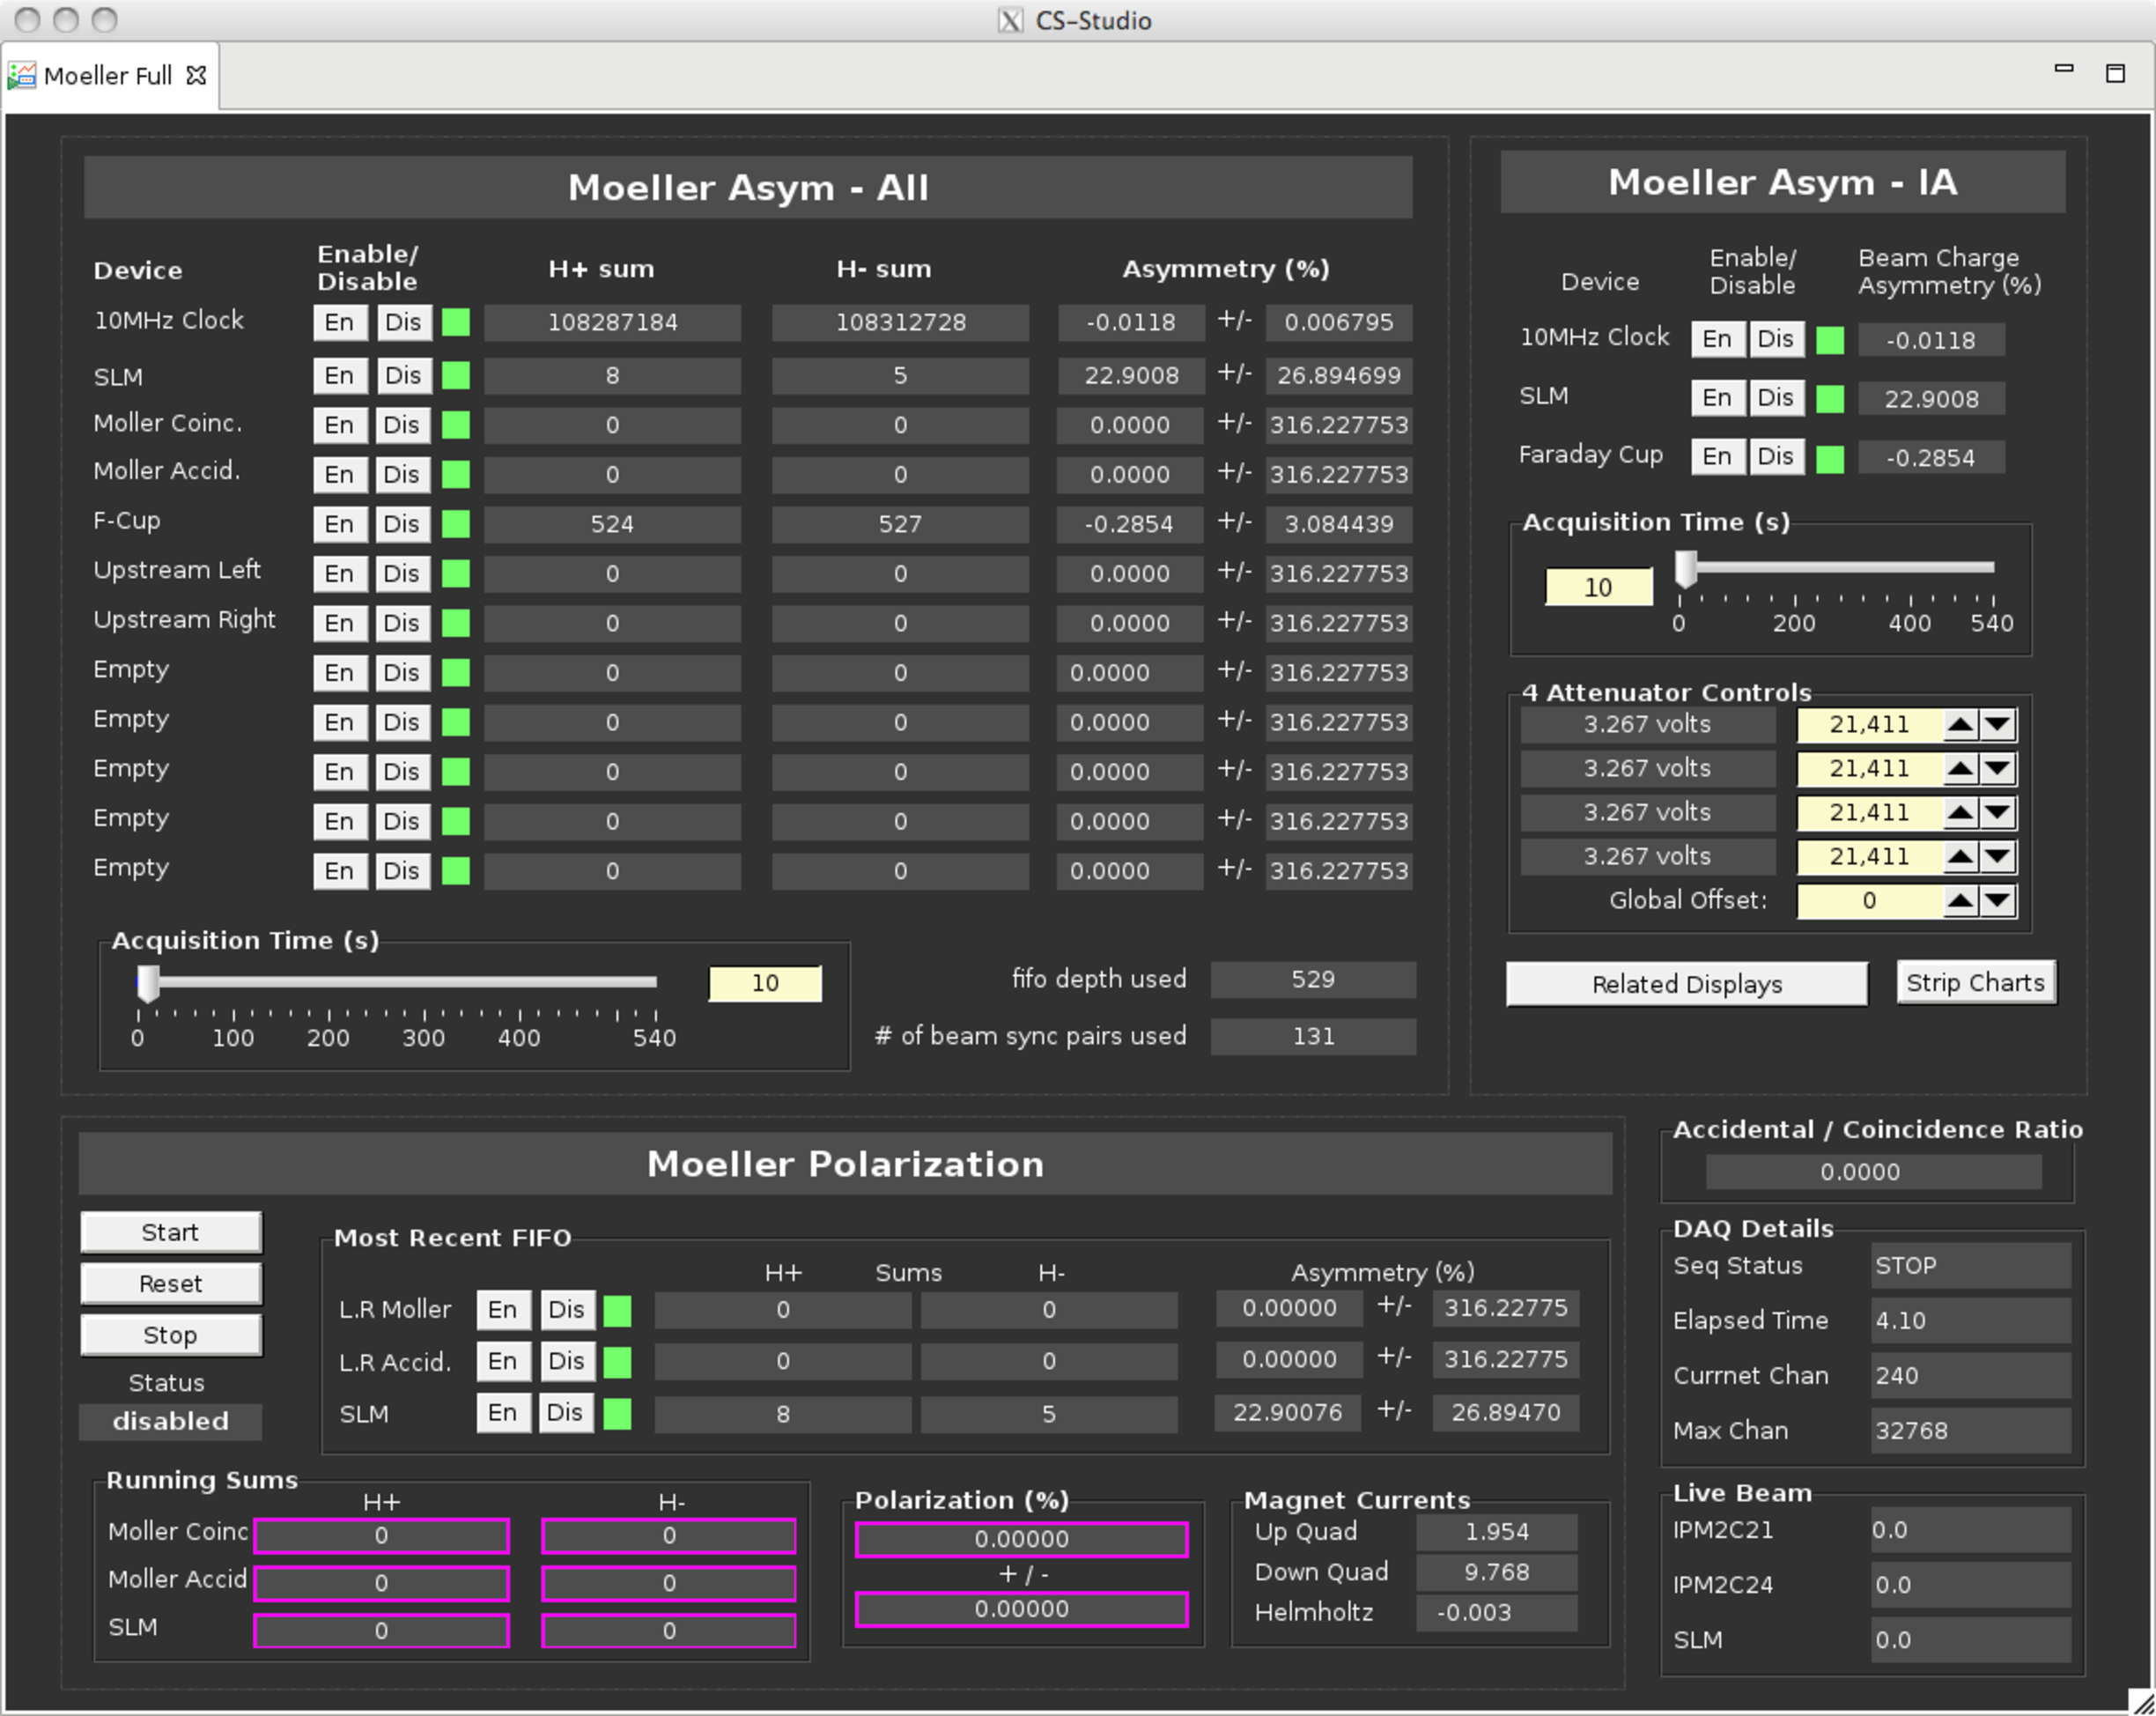
\includegraphics[width=0.8\textwidth]{pics/moller_asym_all.pdf}
\caption{The main M{\o}ller Epics expert GUI.}
\label{fig:mainmoller}
\end{center}
\end{figure}

\item The control for M{\o}ller quadrupole power supplies are provided in "Moeller Quadrupoles" GUI, see Fig.\ref{fig:moller_quad}. Power supplies will be turned ON and in remote before hall closing. From GUI one should first turn them on by pushing the "PS ON" buttons, then set the desire value for currents in "Current Setpoint" window. For $10.7$ GeV the suggested value for the quadrupoles is $XXXX$ A.

\begin{figure}
\begin{center}
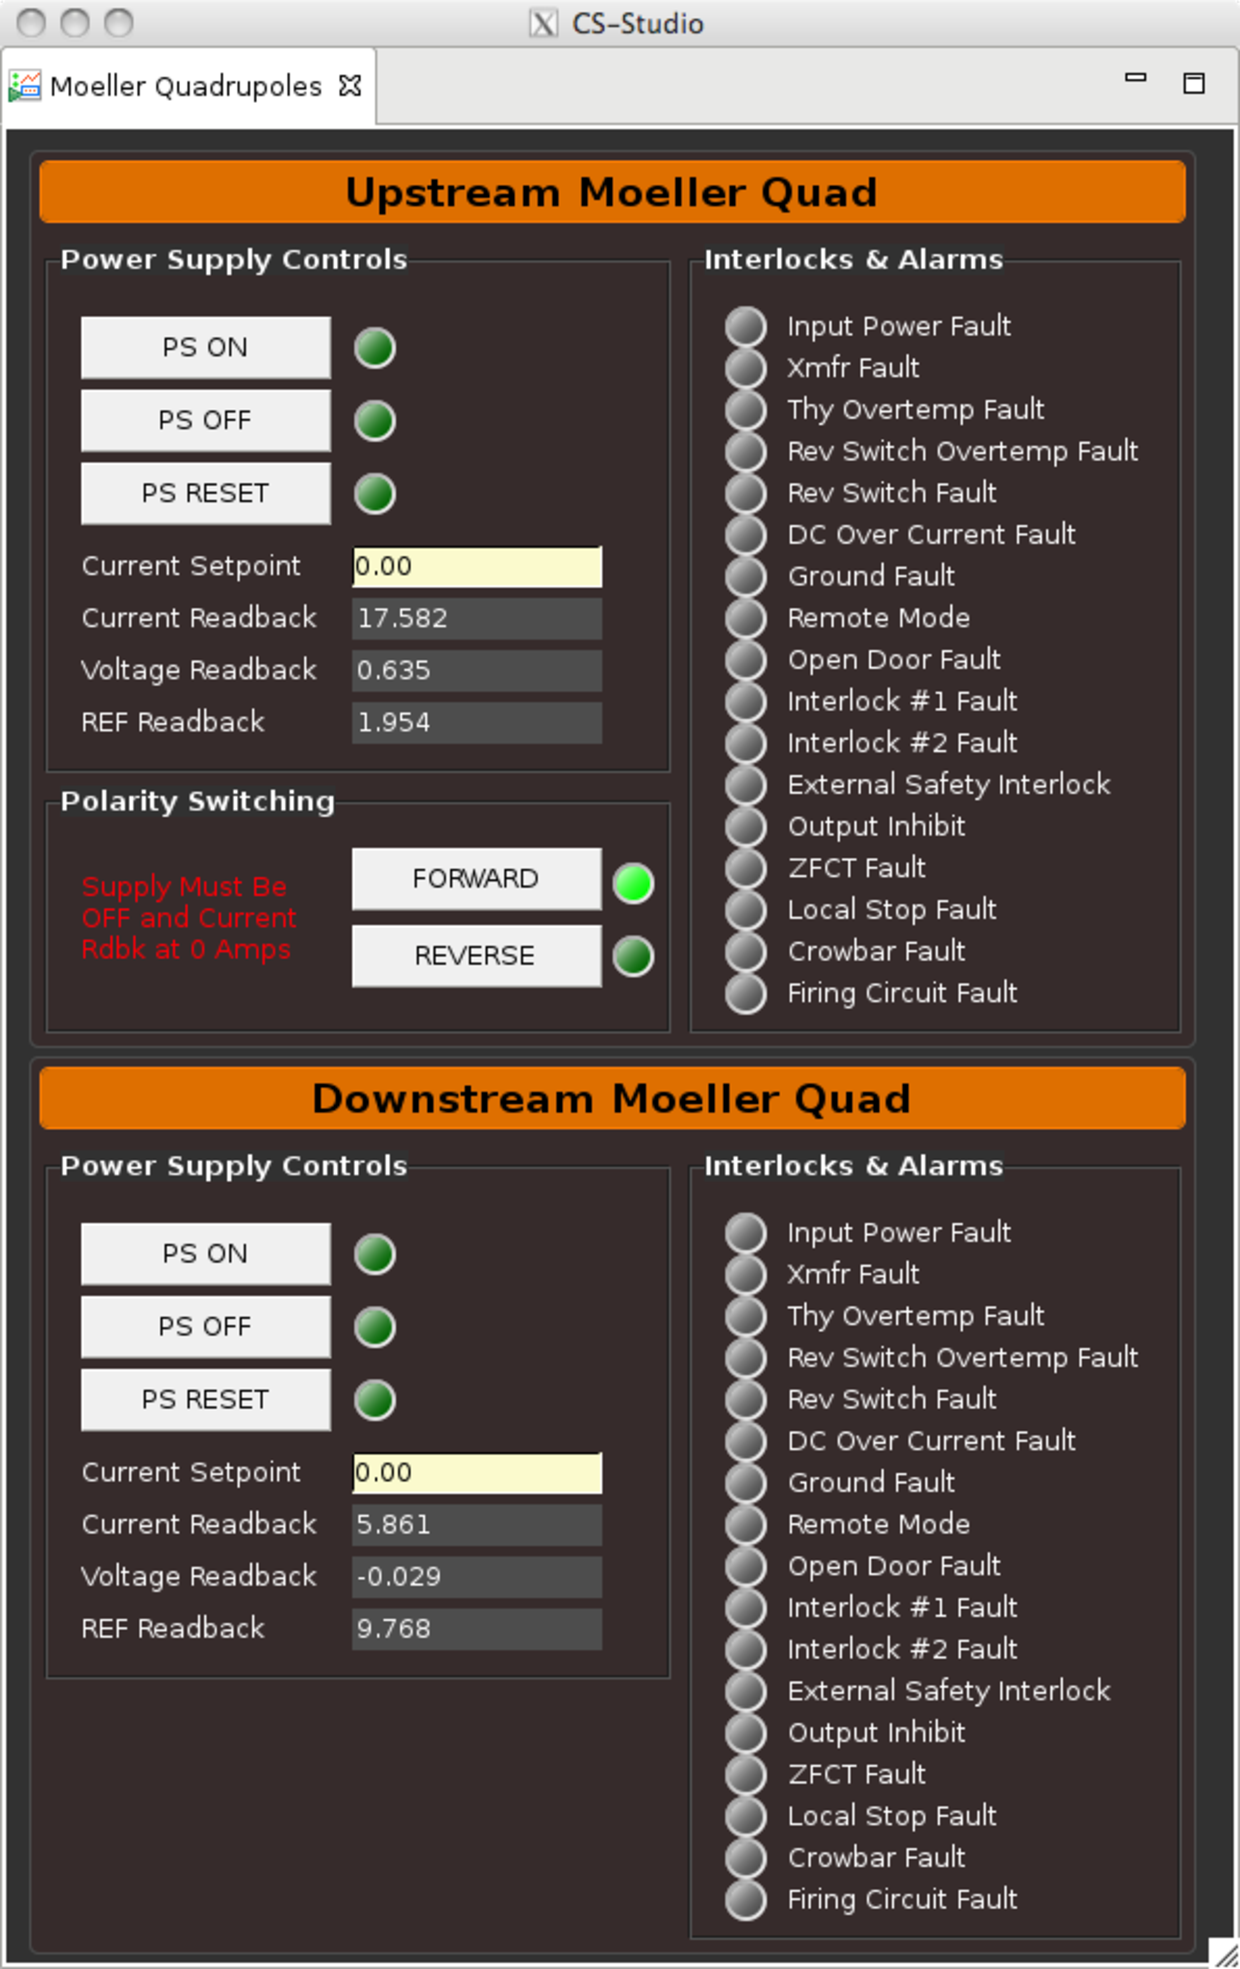
\includegraphics[width=0.75\textwidth]{pics/moller_quad.pdf}
\caption{Control GUI for the M{\o}ller quadrupole power supplies.}
\label{fig:moller_quad}
\end{center}
\end{figure}


%Click \emph{``Configure M{\o}ller Hardware''} button, near the top of the GUI, Figure \ref{fig:moller_epics_setup}. This will start the following sequence of events:

%\begin{enumerate}
%\item SC HV Mainframes will be turned off.
%\item EC HV Mainframes will be turned off.
%\item Helmholtz Magnet will be energized in the Negative polarity.
%\item M{\o}ller Target will be positioned to the \emph{LEFT} target position.
%\item M{\o}ller Quadrupole magnets will be energized
%\item EPICS DAQ will be started
%\end{enumerate}
%\item Watch the text at the top of the GUI for informational guidance.

\item The target is polarized to its saturation by a longitudinal (along the beam) magnetic field generated using pair of Helmholtz coils. It is expected that the target will be saturated at $\sim 1.8$ A current in the coils. The recommended current for M{\o}ller measurement is $X.X$ A. A GUI for power supply of Helmholtz coils, "Moeller Helmholtz PS" see Fig.\ref{fig:moller_helm}, has two controls, button "STATE" defines state of the power supply. Typicaly it will be in "STANDBY" state when is not used. To energize coils first from the menu in "STATE" chose PS ON, then in "Current Setpoint", a white window, write the value, either $X.X$ or $-X.X$. Beam polarization measurements with both orientations the Helmholtz field is recommended to check systematics.    

\begin{figure}
\begin{center}
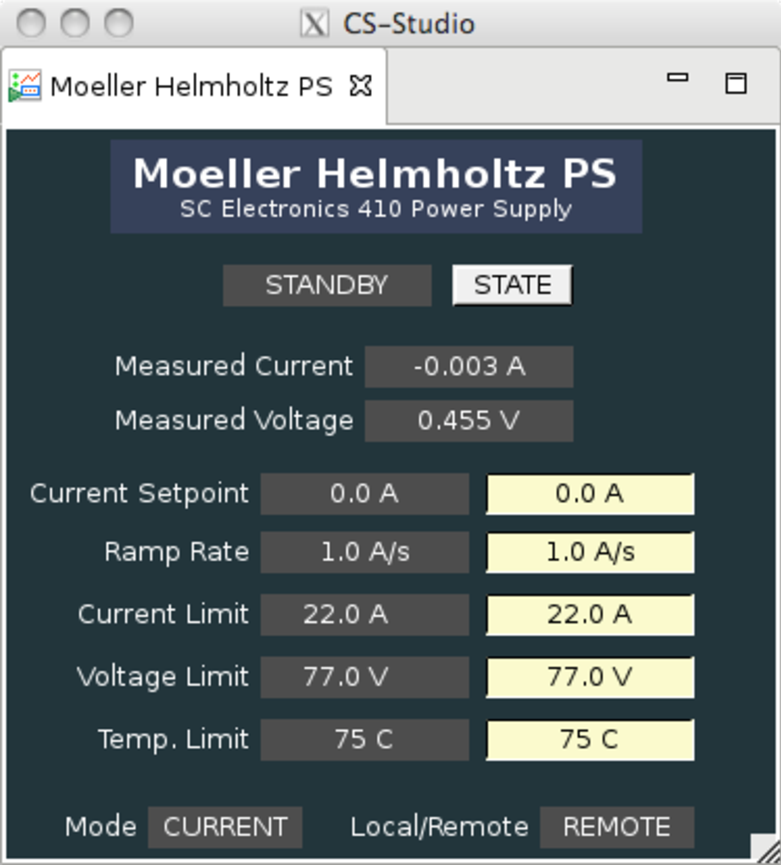
\includegraphics[width=0.65\textwidth]{pics/moller_helmholtz.pdf}
\caption{Control GUI for the M{\o}ller target Helmholtz coils power supply.}
\label{fig:moller_helm}
\end{center}
\end{figure}
%\clearpage

\item a target control GUI, Fig.\ref{fig:moller_target}, allows to position desired target on the beam. Left target is the recommended target for the measurements.

\begin{figure}
\begin{center}
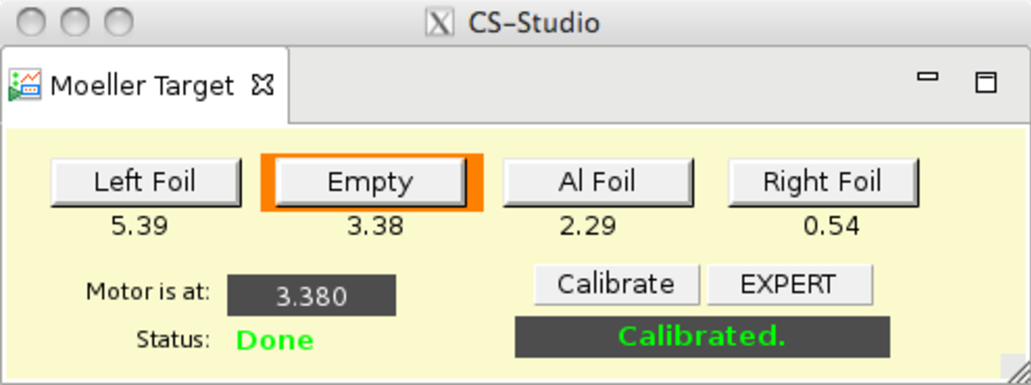
\includegraphics[width=0.65\textwidth]{pics/moller_target.pdf}
\caption{Control GUI for the M{\o}ller target.}
\label{fig:moller_target}
\end{center}
\end{figure}

\end{enumerate}
%
%\clearpage

\item Once the tagger magnet is energized, M{\o}ller setup is UP and ready, request the beam current as specify for the given energy M{\o}ller measurements to be delivered\footnote{The optimal beam current is a function of beam energy.
More specific information may be available on the white board in the
counting house or in the run period specific documentation on the run wiki. Regardless
of what currents are specified on the white board or in this document,
the ratio $Left\otimes Right$ accidentals to the true coincidence
rate should be kept below 5\%. It may be necessary to adjust the
HV on the Left and Right PMT's to achieve a low accidental rate, while
maintaining a reasonable true rate.}, 
as measured by 2C21 nA BPM and/or SLM. Do
not use 2C24A since that BPM is located downstream of the M{\o}ller setup. For $\sim 11$ GeV beam, if beam conditions are normal, as expected, the beam current should be $15$ nA. 

\end{enumerate}

\subsubsection{Data Taking}
\indent
\begin{itemize}
\item 
To start a new run when DAQ is still running hit the "Reset" button on "Moeller Asym - All" GUI. If run was stoped hit the "Start" then "Reset". 
\item Run is complete when the error on the beam polarization on the GUI is below $\le 1.5\%$ absolute. Typically it takes about $45$ min to $60$ min to get the required accuracy (beam condition dependent). 
\item Make measurements with both positions of the half-wave plate,  "IN" and "OUT" (start the first measurement with whichever position it is, then do the second measurement with the other setting). 
\item If needed perform measurements with both polarity of the Helmholtz coils. 
\item Log every measurement by sending "Moeller Asym - All" GUI to logbook together with main scaler GUI to document beam currents, beam position, and halo counter rates. 
\end{itemize}

\subsubsection{Backing off M{\o}ller setup out\label{moller cblose out}}

When done with the measurements:
\begin{itemize}
\item Do not forget to make a log entry including all details and the GUI! 

\item Request MCC to take the beam away and \textbf{de-gauss the tagger
magnet if the next step is to send the beam to Faraday cup (usually it is).}

\item Turn off quadrupoles by setting $0$ in "Current Setpoint"s and then when current readback is at $\sim 0$ A push "PS OFF" button

\item Turn off Helmholtz coils by setting $0$ in the current "Current Setpoint" and change "STSTE" to "STANDBY" when "Measured Current" is $\sim 0$

\item Retract the target by pushing "Empty" button on the target GUI

\item Once tagger magnet is degaussed, restore beam to the Faraday Cup.

\item Turn ON CLAS12
\end{itemize}



%\subsubsubsection{Tips}

%\begin{enumerate}
%\item During a M{\o}ller run the upstream PMTs labeled \char`\"{}up\char`\"{} and \char`\"{}down\char`\"{} may get activated. The half life is around 20 Minutes.~ MCC should ignore those PMTs for at least an hour. 
%\item MOLLER QUADS.~ At times the moller quads will not turn on.~ Using the Moller expert screens controls you can try a few things to get them on first try to click the \char`\"{}RESET\char`\"{} and \char`\"{}ON\char`\"{} buttons.~ Then you could try to click the \char`\"{}OFF\char`\"{} and then \char`\"{}ON\char`\"{} buttons.~ The readback value of the current should be close to the entered set value.
%\item Steering:~ Based on the beam tune, the moller quads may substantially deflect the beam.~ A deflection of 5 mm has been observed.~ 
%\item If the Moller PMT's do not come ON, try to reset them using the beamline HV GUI.
%\end{enumerate}

